\title{Aula 15 - IDS/IPS}

\author{Prof. Gabriel Rodrigues Caldas de Aquino}

\institute
{
    Instituto de Computação \\
    Universidade Federal do Rio de Janeiro\\
    gabrielaquino@ic.ufrj.br% Your institution for the title page
}
\date{Compilado em: \\ \today} % Date, can be changed to a custom date

%----------------------------------------------------------------------------------------
%    PRESENTATION SLIDE
%----------------------------------------------------------------------------------------



\begin{frame}
    % Print the title page as the first slide
    \titlepage
\end{frame}

\begin{frame}{A Ameaça: Intrusos e a Necessidade de Defesa}
    \begin{itemize}
        \item Uma das principais ameaças à segurança são os \textbf{intrusos}.



        \item Boa parte das violações são feitas por \textbf{outsiders}
        \item Mas existem algumas violações feitas por \textbf{insiders}.
        \item \textbf{Porém:} Insiders podem ser muito mais perigosos.


        \item \textbf{Preocupação:} Ataques \textbf{direcionados} a indivíduos e seus sistemas de TI.


        \item \textbf{Implicação:}
              \begin{itemize}
                  \item Ataques direcionados podem \textit{burlar} as defesas de perímetro (ex: Firewalls).
                  \item É necessário estratégias de \textbf{Defesa em Profundidade}.
              \end{itemize}
    \end{itemize}
\end{frame}

\begin{frame}{Classes de Intrusos (Parte 1): Ciber criminosos e Ativistas}
    Entender a \textbf{motivação} dos atacantes auxilia no design da estratégia defensiva.
    \begin{itemize}


        \item \textbf{Classe 1: Ciber criminosos}
              \begin{itemize}
                  \item \textbf{Motivação:} \textbf{Recompensa Financeira}.
                  \item \textbf{Atividades:} Roubo de identidade, roubo de credenciais financeiras, espionagem corporativa, roubo ou sequestro de dados.
                  \item \textbf{Perfil:} Organizam-se em fóruns \textit{underground} (ex: DarkMarket) para trocar dados e coordenar ataques.
              \end{itemize}

        \item \textbf{Classe 2: Ativistas}
              \begin{itemize}
                  \item \textbf{Motivação:} \textbf{Causas sociais ou políticas}.
                  \item \textbf{Nível de Habilidade:} Frequentemente baixo.
                  \item \textbf{Atividades:} Promover a causa através de \textit{website defacement}, DoS, ou vazamento de dados.
                  \item \textbf{Exemplos:} Anonymous, LulzSec, Manning, Snowden.
              \end{itemize}
    \end{itemize}
\end{frame}

\begin{frame}{Classes de Intrusos (Parte 2): APTs e Outros}
    \begin{itemize}
        \item \textbf{Classe 3: APTs}
              \begin{itemize}
                  \item \textbf{Quem são?} Grupos de hackers \textbf{patrocinados por governos}.
                  \item \textbf{Motivação:} Conduzir \textbf{espionagem} ou \textbf{sabotagem}.
                  \item \textbf{Alias:} \textbf{APTs (Advanced Persistent Threats)} – devido à natureza \textbf{secreta} e \textbf{persistência} por longos períodos.
                  \item \textbf{Escopo:} Generalizado (China, Rússia, EUA, UK, etc.).
              \end{itemize}

        \item \textbf{Classe 4: Outros}
              \begin{itemize}
                  \item \textbf{Hackers Clássicos:}
                        \begin{itemize}
                            \item \textbf{Motivação:} Desafio técnico, ou estima e reputação no grupo.
                            \item Ex: Responsáveis por descobrir novas vulnerabilidades, como buffer overflow.
                        \end{itemize}
                  \item \textbf{Hobby Hackers:}
                        \begin{itemize}
                            \item Usam \textit{attack toolkits} (ferramentas prontas) para explorar.
                            \item Potencialmente podem ser recrutados pelas outras classes.
                        \end{itemize}
              \end{itemize}
    \end{itemize}
\end{frame}

\begin{frame}{Exemplos de Intrusão (NIST SP 800-61) - Parte 1}

    O NIST SP 800-61 (Guia de Resposta a Incidentes) lista os seguintes exemplos de intrusão:
    \begin{itemize}

        \item Realizar um comprometimento \textit{root} remoto de um servidor de e-mail.

        \item Pichar (defacing) um servidor Web.

        \item Adivinhar e quebrar senhas.

        \item Copiar um banco de dados contendo números de cartão de crédito.

        \item Visualizar dados sensíveis (folha de pagamento, registros médicos) sem autorização.
    \end{itemize}
\end{frame}

\begin{frame}{Exemplos de Intrusão (NIST SP 800-61) - Parte 2}
    \begin{itemize}
        \item Executar um \textit{packet sniffer} em uma estação de trabalho para capturar nomes de usuário e senhas.

        \item Usar um erro de permissão em um servidor FTP anônimo para distribuir software pirata e arquivos de música.

        \item Acessar sistema inseguro e obter acesso à rede interna.

        \item \textbf{Engenharia Social}

    \end{itemize}
\end{frame}

\begin{frame}{O Papel e as Limitações do IDS/IPS}
    \begin{itemize}

        \item \textbf{IDS: Sistemas de Detecção de Intrusão}
        \item \textbf{IPS: Sistemas de Prevenção de Intrusão}


        \item \textbf{Onde funcionam bem:}
              \begin{itemize}
                  \item São razoavelmente eficazes contra ataques \textbf{conhecidos} e \textbf{menos sofisticados}.
                  \item Ex: Ataques de grupos ativistas ou golpes de e-mail em larga escala.
              \end{itemize}

        \item \textbf{Onde falham:}
              \begin{itemize}
                  \item São \textbf{menos eficazes} contra ataques sofisticados e direcionados (ex: cibercriminosos ou APTs patrocinados pelo Estado).
                  \item \textit{Por quê?} Esses atacantes usam \textbf{\textit{zero-day exploits}} e sabem como \textbf{obscurecer} suas atividades no sistema.
              \end{itemize}

        \item \textbf{Defesa em Profundidade}
              \begin{itemize}
                  \item O IDS/IPS precisa ser parte de uma estratégia de \textbf{Defesa em Profundidade}. Incluindo criptografia, trilhas de auditoria, autenticação forte e gerenciamento ativo de segurança.
              \end{itemize}
    \end{itemize}
\end{frame}

\begin{frame}{Comportamento do Intruso: Metodologia de Ataque}
    Padrões de comportamento dos intrusos mudam e constantemente

    \begin{itemize}
        \item \textbf{Porém existe} uma metodologia de ataque comum:
              \begin{itemize}
                  \item Phishing $\rightarrow$ Instalação de Malware $\rightarrow$ Roubo de Credenciais $\rightarrow$ Comprometimento.
              \end{itemize}
    \end{itemize}
    \textbf{Etapas:}

    \begin{itemize}


        \item \textbf{1. Aquisição de Alvo e Coleta de Informações}
              \begin{itemize}
                  \item Ossint - Open source intelligence
                  \item Usa informações publicamente disponíveis (técnicas ou não)
                  \item Uso de ferramentas de mapeamento de rede
                  \item \textbf{Objetivo}: Identificar e caracterizar os sistemas-alvo.
              \end{itemize}

        \item \textbf{2. Acesso Inicial}
              \begin{itemize}
                  \item Explorando uma vulnerabilidade de rede remota.
                  \item Explorando credenciais de autenticação fracas.
                  \item Instalando malware (via \textbf{engenharia social} ou \textbf{download direcionado}).
              \end{itemize}
    \end{itemize}
\end{frame}

\begin{frame}{Metodologia de Ataque (Continuação)}
    \begin{itemize}
        \item \textbf{3. Escalação de Privilégio}
              \begin{itemize}
                  \item Ações tomadas \textbf{dentro} do sistema \textbf{após o acesso inicial}.
                  \item Explora vulnerabilidades de acesso \textit{local}.
                  \item \textbf{Objetivo:} Aumentar os privilégios disponíveis para o atacante, permitindo que ele atinja seus objetivos no sistema-alvo.
              \end{itemize}

        \item \textbf{4. Coleta de Informações ou Exploração do Sistema}
              \begin{itemize}
                  \item Ações do atacante para acessar ou modificar informações/recursos no sistema.
                  \item Pode incluir mudar para outro sistema-alvo (\textbf{movimentação lateral}).
              \end{itemize}
    \end{itemize}
\end{frame}

\begin{frame}{Metodologia de Ataque (Finalização)}
    \begin{itemize}
        \item \textbf{5. Manutenção do Acesso}
              \begin{itemize}
                  \item Ações para permitir acesso contínuo (persistência) pelo atacante.
                  \item Instalação de \textbf{backdoors} ou outro software malicioso.
                  \item Adição de credenciais de autenticação "secretas" .
                  \item Outras mudanças de configuração no sistema.
              \end{itemize}

        \item \textbf{6. Apagando Rastros}
              \begin{itemize}
                  \item O atacante desabilita ou edita \textbf{logs de auditoria} para remover evidências da atividade de ataque.
                  \item Usa \textbf{rootkits} e outras medidas para esconder arquivos ou códigos instalados secretamente.
              \end{itemize}
    \end{itemize}
\end{frame}

\begin{frame}{Examplos de Comportamento do Intruso}
    \begin{itemize}
        \item \textbf{(a) Aquisição de Alvo e Coleta de Informações}
              \begin{itemize}
                  \item Explorar site corporativo (estrutura, pessoal, S.O.).
                  \item Usar DNS lookup (\texttt{dig}, \texttt{host}) e banco de dados \texttt{WHOIS}.
                  \item Mapear serviços de rede (\texttt{NMAP}).
                  \item Enviar e-mail de "sondagem" (ex: SAC) para analisar a resposta (tipo de cliente/servidor de e-mail).
                  \item Identificar serviços vulneráveis (ex: um CMS Web).
              \end{itemize}

        \item \textbf{(b) Acesso Inicial}
              \begin{itemize}
                  \item \textit{Brute force} (adivinhação) de senha (ex: do CMS).
                  \item Explorar uma vulnerabilidade em um plugin (ex: do CMS) para ganhar acesso ao sistema.
                  \item Enviar e-mail de \textit{spear-phishing} direcionado (com link para um \textit{exploit} de navegador).
              \end{itemize}
    \end{itemize}
\end{frame}
\begin{frame}{Examplos de Comportamento do Intruso}
    \begin{itemize}
        \item \textbf{(c) Escalação de Privilégio (Privilege Escalation)}
              \begin{itemize}
                  \item Escanear o sistema por aplicações com \textit{exploits} locais.
                  \item Explorar uma aplicação vulnerável para ganhar privilégios elevados (ex: root/admin).
                  \item Instalar \textit{sniffers} para capturar senhas de administrador na rede.
                  \item Usar a senha de admin capturada para acessar informação privilegiada.
              \end{itemize}

        \item \textbf{(d) Coleta de Informações ou Exploração do Sistema}
              \begin{itemize}
                  \item Escanear arquivos em busca da informação desejada (ex: dados financeiros, PII).
                  \item Transferir um grande número de documentos para um repositório externo (exfiltração de dados).
                  \item Usar senhas (capturadas) para acessar outros servidores na rede (movimentação lateral).
              \end{itemize}
    \end{itemize}
\end{frame}
\begin{frame}{Examplos de Comportamento do Intruso}
    \begin{itemize}
        \item \textbf{(e) Manutenção de Acesso }
              \begin{itemize}
                  \item Instalar uma ferramenta de administração remota (RAT) ou \textit{rootkit} com um \textit{backdoor} para acesso futuro.
                  \item Usar a senha de administrador (capturada) para acessar a rede posteriormente (persistência).
                  \item Modificar ou desabilitar programas de antivírus (AV) ou IDS rodando no sistema para evitar detecção.
              \end{itemize}

        \item \textbf{(f) Apagando Rastros }
              \begin{itemize}
                  \item Usar um \textit{rootkit} para esconder os arquivos (ex: RAT, sniffers) instalados no sistema.
                  \item Editar arquivos de log (\textit{logfiles}) para remover as entradas (evidências) geradas durante a intrusão.
              \end{itemize}
    \end{itemize}
\end{frame}

\begin{frame}{Detecção de Intrusão (Intrusion Detection): Definições}
    \begin{itemize}
        \item \textbf{Intrusão de Segurança:}
              \begin{itemize}
                  \item Um ato \textbf{não autorizado} de \textbf{burlar (bypassing)} os mecanismos de segurança de um sistema.
              \end{itemize}

        \item \textbf{Detecção de Intrusão :}
              \begin{itemize}
                  \item Uma função de hardware ou software que \textbf{coleta e analisa} informações de várias áreas (dentro de um computador ou rede).
                  \item \textbf{Objetivo:} Identificar possíveis intrusões de segurança.
              \end{itemize}
    \end{itemize}
\end{frame}

\begin{frame}{Componentes Lógicos de um IDS}
    \begin{itemize}
        \item Um IDS (Intrusion Detection System) é composto por três componentes lógicos:

        \item \textbf{1. Sensores }
              \begin{itemize}
                  \item Responsáveis por \textbf{coletar dados}.
                  \item A entrada pode ser qualquer parte do sistema que contenha evidência de intrusão
                  \item Ex: pacotes de rede, arquivos de log, system calls.
                  \item Os sensores coletam e encaminham esta informação para o Analisador.
              \end{itemize}

        \item \textbf{2. Analisadores }
              \begin{itemize}
                  \item Recebem a entrada de um ou mais Sensores.
                  \item A saída \textbf{determina se uma intrusão ocorreu}.
                  \item Pode incluir evidências e orientações sobre ações.
                  \item Os dados dos sensores também podem ser armazenados para análise futura.
              \end{itemize}

        \item \textbf{3. Interface de Usuário }
              \begin{itemize}
                  \item Permite ao administrador \textbf{visualizar} o sistema ou \textbf{controlar o seu comportamento}.

              \end{itemize}
    \end{itemize}
\end{frame}

\begin{frame}{Classificação de IDSs (Baseado na Fonte de Dados)}
    \textbf{Arquitetura:}


    \begin{itemize}
        \item \textbf{Simples:} Um IDS com um único sensor e analisador - Ex:  um HIDS ou  NIDS.
        \item \textbf{Distribuída:} Uso de \textbf{múltiplos sensores} em vários hosts e dispositivos de rede, enviando informações para um \textbf{analisador centralizado}.
    \end{itemize}

    \textbf{Classificação (Fonte e Tipo de Dados):}
    \begin{itemize}
        \item \textbf{1. Host-based IDS (HIDS)}
              \begin{itemize}
                  \item \textbf{O que monitora?} As características de um \textbf{único host} e os eventos ocorrendo nele.
                  \item \textit{Exemplos:} Identificadores de processo (PIDs), \textit{system calls} (chamadas de sistema).
              \end{itemize}

        \item \textbf{2. Network-based IDS (NIDS)}
              \begin{itemize}
                  \item \textbf{O que monitora?} O \textbf{tráfego de rede} de segmentos ou dispositivos específicos.
                  \item \textit{Exemplos:} Analisa tráfego da rede para identificar atividades suspeitas.
              \end{itemize}

        \item \textbf{3. Distributed ou Hybrid IDS (Distribuído/Híbrido)}
              \begin{itemize}
                  \item \textbf{O que faz?} Combina informações de vários sensores (HIDS e/ou NIDS) em um analisador central.
                  \item \textit{Vantagem:} Consegue identificar e responder melhor à atividade de intrusão.
              \end{itemize}
    \end{itemize}
\end{frame}

\begin{frame}{Princípios Básicos: Motivações para o IDS}
    \begin{itemize}
        \item Autenticação, Controle de Acesso e Firewalls ajudam a combater intrusões.
        \item A \textbf{Detecção de Intrusão (IDS)} é outra linha de defesa, motivada por várias considerações:

        \item \textbf{1. Detecção Rápida }
              \begin{itemize}
                  \item Se a intrusão for detectada rápido o suficiente, o intruso pode ser \textbf{ejetado} do sistema \textit{antes} de causar danos ou comprometer dados.
                  \item Mesmo se não for a tempo de "preempt" (impedir), quanto mais cedo a detecção, menor o dano e mais rápida a recuperação.
              \end{itemize}

        \item \textbf{2. Efeito desencorajador}
              \begin{itemize}
                  \item Um IDS eficaz pode desencorajar ataques, atuando assim para \textbf{prevenir} intrusões.
              \end{itemize}

        \item \textbf{3. Coleta de Informações}
              \begin{itemize}
                  \item A detecção permite a coleta de informações sobre \textbf{técnicas de intrusão}.
                  \item Essas informações podem ser usadas para fortalecer as medidas de \textbf{prevenção} (ex: regras de firewall, patches).
              \end{itemize}
    \end{itemize}
\end{frame}

\begin{frame}{Princípios Básicos: A Suposição Fundamental do IDS}
    \begin{itemize}
        \item \textbf{A Suposição:}
              \begin{itemize}
                  \item A detecção de intrusão baseia-se na suposição de que o comportamento do \textbf{intruso} difere do comportamento de um \textbf{usuário legítimo} de maneiras que podem ser \textbf{quantificadas}.
              \end{itemize}

        \item \textbf{O Desafio (A Realidade):}
              \begin{itemize}
                  \item Não podemos esperar que haja uma distinção \textbf{nítida (crisp) e exata} entre um ataque e o uso normal dos recursos.
              \end{itemize}

        \item \textbf{A Consequência (Falsos Positivos/Negativos):}
              \begin{itemize}
                  \item Devemos esperar que haverá alguma \textbf{sobreposição (overlap)} entre o comportamento legítimo e o comportamento de ataque.
                  \item (O trabalho do Analisador é minimizar essa sobreposição).
              \end{itemize}
    \end{itemize}
\end{frame}

\begin{frame}{O Desafio Central do IDS: O "Trade-Off"}
    \begin{itemize}
        \item O comportamento típico de um intruso e de um usuário autorizado não são perfeitamente distintos; existe uma \textbf{sobreposição (overlap)}.

        \item \textbf{O Dilema (Compromisso):}
              \begin{itemize}
                  \item \textbf{1. Interpretação "Frouxa" (Loose):}
                        \begin{itemize}
                            \item Tenta capturar o máximo de intrusos.
                            \item \textbf{Resultado:} Leva a um alto número de \textbf{Falsos Positivos} (Falsos Alarmes), onde usuários autorizados são identificados como intrusos.
                        \end{itemize}
                  \item \textbf{2. Interpretação "Restrita" (Tight):}
                        \begin{itemize}
                            \item Tenta limitar os Falsos Positivos.
                            \item \textbf{Resultado:} Leva a um aumento de \textbf{Falsos Negativos} (intrusos não identificados).
                        \end{itemize}
              \end{itemize}

        \item \textbf{O Objetivo Ideal:}
              \begin{itemize}
                  \item A prática do IDS é um "compromisso" (e uma "arte").
                  \item Maximizar a \textbf{Taxa de Detecção} (detectar ataques reais).
                  \item Minimizar a \textbf{Taxa de Falsos Alarmes} (ignorar uso normal).
              \end{itemize}
    \end{itemize}
\end{frame}

\begin{frame}{A Visão Clássica}

    A dificuldade de detecção depende do tipo de intruso:
    \begin{itemize}


        \item \textbf{Detectando Atacantes Externos (Outsiders):}
              \begin{itemize}
                  \item É possível (com confiança razoável) distinguir um atacante externo de um usuário legítimo.
                  \item \textbf{Como?} Padrões de comportamento legítimo podem ser estabelecidos (observando o histórico).
                  \item \textbf{Detecção:} Pode-se detectar \textbf{desvios significativos} (anomalias) desses padrões.
              \end{itemize}

        \item \textbf{Detectando Atacantes Internos (Insiders):}
              \begin{itemize}
                  \item (Um usuário legítimo agindo de forma não autorizada).
                  \item Anderson concluiu que esta é a tarefa \textbf{mais difícil}.
                  \item \textbf{Por quê?} A distinção entre o comportamento "anormal" (malicioso) e "normal" (legítimo) de um insider pode ser \textbf{muito pequena}.
                  \item \textbf{Conclusão:} A busca \textit{apenas} por anomalias seria \textbf{insuficiente} para detectar insiders.
                  \item \textbf{Solução (sugerida):} O comportamento do insider pode ser detectável através de uma \textbf{definição inteligente} de condições (regras) que sugerem uso não autorizado.
              \end{itemize}
    \end{itemize}
\end{frame}

\begin{frame}{O Desafio Prático do IDS}
    \begin{itemize}
        \item \textbf{O Objetivo Duplo (e Conflitante):}
              \begin{itemize}
                  \item \textbf{1. Alta Taxa de Detecção:} Detectar uma porcentagem substancial de intrusões (senão, o IDS gera uma \textit{falsa sensação de segurança}).
                  \item \textbf{2. Baixa Taxa de Falsos Alarmes:} Se os falsos positivos (alarmes) forem frequentes, os gerentes \textbf{passarão a ignorar os alarmes} ou perderão muito tempo analisando-os.
              \end{itemize}

        \item \textbf{A Falácia da Taxa-Base (Base-Rate Fallacy):}
              \begin{itemize}
                  \item É \textbf{extremamente difícil} atingir os dois objetivos.
                  \item \textbf{O Problema:} O número real de \textbf{intrusões} (taxa-base) é \textbf{muito baixo} em comparação com o número de \textbf{usos legítimos} (normal).
                  \item \textbf{A Consequência:} A menos que o teste (o IDS) seja \textit{extremamente discriminatório} (quase perfeito), a taxa de falsos alarmes será \textbf{alta}.
                  \item \textbf{O desafio está aqui}
              \end{itemize}
    \end{itemize}
\end{frame}

\begin{frame}{Requisitos de um IDS - Parte 1}

    Um IDS deve:
    \begin{itemize}


        \item \textbf{1. Rodar continuamente} com mínima supervisão humana.

        \item \textbf{2. Ser tolerante a falhas}, ou seja, capaz de se recuperar de \textit{crashes} e reinicializações.

        \item \textbf{3. Resistir à subversão.} O IDS deve ser capaz de monitorar a si mesmo e detectar se foi modificado por um atacante.

        \item \textbf{4. Impor um \textit{overhead} mínimo} no sistema onde está rodando.

        \item \textbf{5. Ser configurável} de acordo com as políticas de segurança do sistema que está sendo monitorado.
    \end{itemize}
\end{frame}

\begin{frame}{Requisitos de um IDS - Parte 2}sobrecarga
    \begin{itemize}
        \item \textbf{6. Ser capaz de se adaptar} a mudanças no comportamento do sistema e dos usuários ao longo do tempo.

        \item \textbf{7. Ser capaz de escalar } para monitorar um grande número de hosts.

        \item \textbf{8. Evitar parada completa} do serviço, ou seja, se alguns componentes pararem, o resto deve ser afetado o mínimo possível.

        \item \textbf{9. Permitir reconfiguração dinâmica}, ou seja, a capacidade de reconfigurar o IDS sem ter que reiniciá-lo.
    \end{itemize}
\end{frame}

\begin{frame}{Abordagens de Análise de um IDS}
    Os IDSs usam duas abordagens:
    \begin{itemize}


        \item \textbf{1. Detecção de Anomalia}


        \item \textbf{2. Detecção por Assinatura ou Heurística }

    \end{itemize}
\end{frame}



\begin{frame}{Abordagens de Análise de um IDS}

    \begin{itemize}


        \item \textbf{1. Detecção de Anomalia}
              \begin{itemize}
                  \item \textbf{Como funciona?} Envolve a coleta de dados sobre o comportamento de \textbf{usuários legítimos} ao longo do tempo (criando uma "linha de base" do que é \textbf{normal}).
                  \item \textbf{Análise:} O comportamento \textit{atual} observado é então analisado.
                  \item \textbf{Decisão:} O IDS determina se o comportamento atual é de um usuário legítimo ou se é uma \textbf{anomalia} desse padrão, indicando um intruso.
              \end{itemize}


    \end{itemize}
\end{frame}




\begin{frame}{Abordagem de Análise: Detecção de Anomalia (Definição)}
    Duas fases:
    \begin{itemize}

        \item \textbf{1. Fase de Treinamento}
              \begin{itemize}
                  \item Desenvolve um \textbf{modelo} do comportamento legítimo (normal) do usuário.
                  \item Como? Coletando e processando dados dos sensores durante a operação normal do sistema.
                  \item (Pode ocorrer em momentos distintos ou ser um processo contínuo de evolução do modelo).
              \end{itemize}

        \item \textbf{2. Fase de Detecção}
              \begin{itemize}
                  \item O comportamento \textbf{atual} observado é comparado com o modelo (normal).
                  \item O comportamento é então classificado como \textbf{legítimo} ou \textbf{anômalo} (suspeito).
              \end{itemize}
    \end{itemize}
\end{frame}

\begin{frame}{Detecção de Anomalia: Categorias de Classificação}
    Temos três abordagens:
    \begin{itemize}


        \item \textbf{1. Estatística}
              \begin{itemize}
                  \item Análise do comportamento observado usando modelos (univariados, multivariados, time-series) das métricas.
              \end{itemize}

        \item \textbf{2. Baseada em Conhecimento}
              \begin{itemize}
                  \item Usa um \textbf{sistema especialista} (expert system) que classifica o comportamento de acordo com um conjunto de \textbf{regras} que modelam o comportamento legítimo.
              \end{itemize}

        \item \textbf{3. Aprendizado de Máquina (Machine-learning)}
              \begin{itemize}
                  \item Determina \textbf{automaticamente} um modelo de classificação adequado a partir dos dados de treinamento, usando técnicas de mineração de dados.
              \end{itemize}


    \end{itemize}
\end{frame}

\begin{frame}{Abordagem 1: Estatística}
    Desenvolve um \textbf{perfil estatístico} das métricas observadas.
    \begin{itemize}
        \item \textbf{Uso de:}
              \begin{itemize}
                  \item \textit{Univariada:} Trata cada métrica como independente (muito "cru" (crude), ineficaz).
                  \item \textit{Multivariada:} Considera correlações entre métricas (melhor discriminação).
                  \item \textit{Séries Temporais (Time-series):} Usa a ordem e o tempo entre eventos (ainda melhor).
              \end{itemize}

        \item \textbf{Vantagens:}
              \begin{itemize}
                  \item Relativa simplicidade e baixo custo computacional.
                  \item Não necessita de suposições (assumptions) sobre o comportamento esperado.
              \end{itemize}

        \item \textbf{Desvantagens:}
              \begin{itemize}
                  \item Dificuldade em selecionar métricas adequadas (balanço de falsos positivos/negativos).
                  \item Nem todos os comportamentos podem ser modelados por esta abordagem.
              \end{itemize}
    \end{itemize}
\end{frame}

\begin{frame}{Abordagem 2: Baseada em Conhecimento}
    \begin{itemize}
        \item Classifica os dados observados usando um \textbf{conjunto de regras} (expert system).

        \item \textbf{Fase de Treinamento:}
              \begin{itemize}
                  \item As regras são desenvolvidas (podendo ser \textbf{manualmente}) para caracterizar os dados de treinamento em classes distintas.
                  \item Pode usar ferramentas formais: máquinas de estado finito, linguagens de descrição.
              \end{itemize}

        \item \textbf{Vantagens:}
              \begin{itemize}
                  \item Robustez e flexibilidade.
              \end{itemize}

        \item \textbf{Desvantagens:}
              \begin{itemize}
                  \item \textbf{Dificuldade e tempo} para desenvolver regras (conhecimento) de alta qualidade.
                  \item Necessidade de \textbf{especialistas humanos} (human experts) para auxiliar no processo.
              \end{itemize}
    \end{itemize}
\end{frame}

\begin{frame}{Abordagem 3: Aprendizado de Máquina (Conceito e Trade-offs)}
    \begin{itemize}
        \item Usa técnicas de \textit{data mining} para desenvolver \textbf{automaticamente} um modelo a partir dos dados de treinamento (normais).

        \item \textbf{Fase de Treinamento (Custo):}
              \begin{itemize}
                  \item Requer \textbf{tempo significativo} e \textbf{altos recursos computacionais}.
              \end{itemize}

        \item \textbf{Fase de Detecção (Eficiência):}
              \begin{itemize}
                  \item Uma vez que o modelo é gerado, a análise subsequente (classificação) é geralmente \textbf{bastante eficiente}.
              \end{itemize}

        \item \textbf{Vantagens:}
              \begin{itemize}
                  \item Flexibilidade e adaptabilidade.
                  \item Capacidade de capturar interdependências complexas entre as métricas.
              \end{itemize}

        \item \textbf{Desvantagens:}
              \begin{itemize}
                  \item Dependência de suposições sobre o comportamento "aceito".
                  \item Taxa de \textbf{falsos alarmes} (false alarm rate) \textbf{inaceitavelmente alta} (atualmente).
                  \item Alto custo de recursos (para treinar).
              \end{itemize}
    \end{itemize}
\end{frame}

\begin{frame}{Abordagem 3: Aprendizado de Máquina - Abordagens}
    Várias abordagens de ML foram tentadas com sucesso variado:

    \begin{itemize}

        \item \textbf{Redes Bayesianas:} Codifica relações probabilísticas.

        \item \textbf{Modelos de Markov:} Modelo com conjuntos de estados interligados por probabilidades de transição.

        \item \textbf{Redes Neurais:} Para classificar dados.

        \item \textbf{Lógica Fuzzy:} Raciocínio é aproximado; pode acomodar incerteza.

        \item \textbf{Algoritmos Genéticos:} Desenvolver regras de classificação.

        \item \textbf{Clusterização e Detecção de Outlier:} Agrupa dados por similaridade; novos dados são classificados como "dentro de um cluster" (normal) ou "outlier" (anomalia).
    \end{itemize}
\end{frame}

\begin{frame}{Abordagens de Análise de um IDS}

    \begin{itemize}




        \item \textbf{2. Detecção por Assinatura ou Heurística }
              \begin{itemize}
                  \item Também conhecida como \textbf{Detecção de Mau Uso }.
                  \item \textbf{Como funciona?} Usa um conjunto de \textbf{padrões maliciosos conhecidos} ou \textbf{regras de ataque}.
                  \item \textbf{Análise:} O comportamento atual é comparado com este conjunto de regras/assinaturas.
                  \item \textbf{Decisão:} Se houver uma correspondência, é considerado um intruso.
              \end{itemize}
    \end{itemize}
\end{frame}


\begin{frame}{Abordagem de Análise: Detecção por Assinatura }
    \begin{itemize}

        \item \textbf{Como Funciona:}
              \begin{itemize}
                  \item Compara os dados coletados com \textbf{padrões conhecidos de dados maliciosos}.
                  \item As assinaturas precisam dar detalhes o suficiente para minimizar falsos alarmes, mas ainda detectar uma fração suficiente de dados maliciosos.
              \end{itemize}

        \item \textbf{Onde é usado:} Amplamente utilizado em produtos antivírus, proxies de varredura de tráfego de rede e NIDS.

        \item \textbf{Vantagens:}
              \begin{itemize}
                  \item Custo relativamente baixo em tempo e uso de recursos.
                  \item Ampla aceitação.
              \end{itemize}

        \item \textbf{Desvantagens:}
              \begin{itemize}
                  \item Esforço significativo necessário para identificar e revisar novos comportamentos para criar assinaturas.
                  \item \textbf{Incapacidade de detectar ataques "zero-day"} onde nenhuma assinatura existe.
              \end{itemize}
    \end{itemize}
\end{frame}

\begin{frame}{Abordagem de Análise: Detecção Heurística}
    \begin{itemize}
        \item \textbf{Como Funciona:}
              \begin{itemize}
                  \item Envolve o uso de \textbf{regras} para identificar ataques \textbf{conhecidos} ou que explorariam \textbf{fraquezas conhecidas}.

                  \item As regras também podem identificar comportamento \textbf{suspeito}, mesmo que esse comportamento esteja dentro dos padrões de uso estabelecidos.
              \end{itemize}

        \item \textbf{Desenvolvimento das Regras:}
              \begin{itemize}
                  \item Abordagem mais frutífera: \textbf{Analisar ferramentas e scripts de ataque} coletados na Internet.
                  \item Suplementado por regras geradas por \textbf{especialistas}.
                  \item As regras são tipicamente específicas para a máquina e o S.O.
              \end{itemize}

        \item \textbf{Exemplo:}
              \begin{itemize}
                  \item O sistema \textbf{SNORT} é um exemplo de um \textbf{NIDS baseado em regras}.
                  \item Existe uma grande coleção de regras para ele detectar uma ampla variedade de ataques de rede.
              \end{itemize}
    \end{itemize}
\end{frame}

\begin{frame}{Host-Based IDS (HIDS): Introdução}
    \begin{itemize}
        \item \textbf{O que é?}
              \begin{itemize}
                  \item O HIDS adiciona uma \textbf{camada especializada de software de segurança} a sistemas vulneráveis ou sensíveis.
                  \item \textit{Exemplos:} Servidores de banco de dados, sistemas administrativos.
              \end{itemize}

        \item \textbf{Função:}
              \begin{itemize}
                  \item Monitora a atividade \textbf{dentro do sistema} de várias maneiras para detectar comportamento suspeito.
              \end{itemize}

        \item \textbf{Propósito Principal:}
              \begin{itemize}
                  \item 1. Detectar intrusões.
                  \item 2. Registrar (log) eventos suspeitos.
                  \item 3. Enviar alertas.
                  \item IDS/IPS
              \end{itemize}


        \item \textbf{Abordagens de Análise:}
              \begin{itemize}
                  \item HIDS usa as duas abordagens:
                  \item Detecção de Anomalia (Anomaly).
                  \item Detecção por Assinatura ou Heurística.
              \end{itemize}
    \end{itemize}
\end{frame}

\begin{frame}{HIDS: Fontes de Dados e Sensores (Parte 1)}
    \begin{itemize}
        \item Um componente fundamental do IDS é o \textbf{sensor} que coleta dados. Um registro da atividade (input) deve ser fornecido ao analisador.
        \item Fontes de dados comuns incluem:

        \item \textbf{1. Rastros de Chamadas de Sistema }
              \begin{itemize}
                  \item Um registro da sequência de \textit{system calls} feitas pelos processos.
                  \item Amplamente reconhecida como a \textbf{fonte de dados preferida} para HIDS.
                  \item \textbf{Vantagem:} Funciona bem em sistemas Unix e Linux.
                  \item \textbf{Desvantagem:} Problemático em sistemas Windows (devido ao uso extensivo de DLLs, que "obscurecem" quais processos usam quais chamadas).
              \end{itemize}

        \item \textbf{2. Registros de Auditoria }
              \begin{itemize}
                  \item A maioria dos S.O. modernos inclui software de "accounting" (auditoria) que coleta informações sobre a atividade do usuário.
                  \item \textbf{Vantagem:} Nenhum software de coleta adicional é necessário.
                  \item \textbf{Desvantagem (1):} Os registros podem não conter a informação necessária ou não estar em um formato conveniente.
                  \item \textbf{Desvantagem (2):} Intrusos podem tentar \textbf{manipular} esses logs para esconder suas ações.
              \end{itemize}
    \end{itemize}
\end{frame}

\begin{frame}{HIDS: Fontes de Dados e Sensores (Parte 2)}
    \begin{itemize}
        \item \textbf{3. Checksums de Integridade de Arquivos }
              \begin{itemize}
                  \item Abordagem comum: Escanear periodicamente \textbf{arquivos críticos} (ex: arquivos de sistema) em busca de mudanças.
                  \item \textbf{Como?} Comparando hash atuais com um registro de valores conhecidos (baseline).
                  \item \textbf{Desvantagem (1):} A necessidade de gerar e proteger os checksums "bons" (baseline).
                  \item \textbf{Desvantagem (2):} A dificuldade de monitorar arquivos que \textit{mudam} (legitimamente) o tempo todo.
              \end{itemize}

        \item \textbf{4. Acesso ao Registro}
              \begin{itemize}
                  \item Uma abordagem usada em sistemas \textbf{Windows}.
                  \item Monitora o acesso ao Registro (dada a quantidade de informação e acesso usados pelos programas).
                  \item \textbf{Desvantagem:} Muito específico do Windows; registrou sucesso limitado.
              \end{itemize}

        \item \textbf{Função Resumida do Sensor:}
              \begin{itemize}
                  \item Coleta dados $\rightarrow$ Filtra (padroniza formato) $\rightarrow$ Encaminha para o Analisador.
              \end{itemize}
    \end{itemize}
\end{frame}

\begin{frame}{HIDS por Anomalia (Sistemas Linux/UNIX)}
    \begin{itemize}
        \item A maioria dos trabalhos em HIDS por anomalia foi feita em UNIX/Linux (dada a facilidade de coletar dados).

        \item \textbf{Fonte de Dados Preferida:} \textbf{Rastros de Chamadas de Sistema} .
              \begin{itemize}
                  \item Logs de auditoria.
              \end{itemize}

        \item \textbf{Por que "System Calls"?}
              \begin{itemize}
                  \item São o meio pelo qual os programas acessam as funções do \textbf{kernel}.
                  \item Fornecem informação \textbf{detalhada} sobre a atividade do processo, permitindo classificar como normal ou anômalo.
              \end{itemize}

    \end{itemize}
\end{frame}

\begin{frame}{HIDS (Linux) - Motores de Decisão }
    \begin{itemize}
        \item Os \textit{system call traces} (coletados) são analisados por um motor de decisão.

        \item \textbf{Abordagem Original (STIDE):}
              \begin{itemize}

                  \item Compara sequências de chamadas observadas com sequências "normais" (do treinamento) para obter uma "taxa de disparidade" (mismatch ratio).
              \end{itemize}

        \item \textbf{Abordagens Alternativas (ML):}
              \begin{itemize}
                  \item Hidden Markov Models (HMM)
                  \item Redes Neurais Artificiais (ANN)
                  \item Support Vector Machines (SVM)
                  \item Extreme Learning Machines (ELM)
              \end{itemize}

        \item \textbf{Performance:}
              \begin{itemize}
                  \item taxa\% detecção, falsos positivos.
                  \item velocidade de detecção.
              \end{itemize}
    \end{itemize}
\end{frame}

\begin{frame}{HIDS: Detecção por Assinatura ou Heurística}
    \begin{itemize}


        \item \textbf{Implementação Comum:} É a base dos \textbf{Antivírus}.
              \begin{itemize}
                  \item Usado em: sistemas cliente (PCs), dispositivos móveis, e incorporado em proxies (e-mail, Web) e NIDS.
              \end{itemize}

        \item \textbf{Como Funciona (Duas Técnicas):}
              \begin{itemize}
                  \item \textbf{1. Assinaturas :}
                        \begin{itemize}
                            \item Um banco de dados de \textbf{padrões de dados} (file signatures) encontrados em malware \textbf{conhecido}.
                        \end{itemize}
                  \item \textbf{2. Heurísticas:}
                        \begin{itemize}
                            \item Um conjunto de \textbf{regras} que caracterizam o \textbf{comportamento} malicioso \textbf{conhecido}.
                        \end{itemize}
              \end{itemize}

        \item \textbf{Vantagem:}
              \begin{itemize}
                  \item \textit{Muito eficiente} para detectar malware \textbf{conhecido}.
              \end{itemize}

        \item \textbf{Desvantagem :}
              \begin{itemize}
                  \item \textbf{NÃO é capaz} de detectar ataques \textbf{"zero-day"} (ataques novos/desconhecidos).
                  \item Pois o novo ataque não corresponde a nenhuma assinatura ou regra conhecida.
              \end{itemize}

        \item \textbf{Uso Principal:}
              \begin{itemize}
                  \item Amplamente utilizado, especialmente em sistemas \textbf{Windows} (que continuam a ser um alvo principal de intrusos).
              \end{itemize}
    \end{itemize}
\end{frame}

\begin{frame}{HIDS Distribuído}
    \begin{itemize}
        \item \textbf{O Foco Tradicional:}
              \begin{itemize}
                  \item O trabalho em HIDS (Host-based) focava-se na operação \textbf{\textit{stand-alone}} (em um único sistema).
              \end{itemize}

        \item \textbf{A Realidade Organizacional:}
              \begin{itemize}
                  \item A organização típica precisa defender uma coleção \textbf{distribuída} de hosts (suportados por uma LAN ou inter-rede).
              \end{itemize}

        \item \textbf{A Evolução (A Defesa Eficaz):}
              \begin{itemize}
                  \item Embora seja possível usar HIDS \textit{stand-alone} em cada host...
                  \item Uma defesa \textbf{mais eficaz} é alcançada através da \textbf{coordenação e cooperação} entre os IDSs pela rede (ou seja, um HIDS Distribuído).
              \end{itemize}
    \end{itemize}
\end{frame}

\begin{frame}{Network-Based IDS (NIDS): Definição e Papel}
    \begin{itemize}
        \item \textbf{O que é um NIDS?}
              \begin{itemize}
                  \item Monitora o tráfego em \textbf{pontos selecionados} de uma rede.
                  \item Examina o tráfego \textbf{pacote a pacote} em tempo real (ou próximo a isso).
                  \item Analisa atividade nos protocolos de Rede (L3), Transporte (L4) e/ou Aplicação (L7).
              \end{itemize}

        \item \textbf{Contraste (NIDS vs. HIDS):}
              \begin{itemize}
                  \item \textbf{NIDS:} Examina o \textit{tráfego de pacotes} \textbf{direcionado aos} sistemas.
                  \item \textbf{HIDS:} Examina a \textit{atividade do usuário e do software} \textbf{dentro de} um host.
              \end{itemize}

        \item \textbf{Papel e Localização:}
              \begin{itemize}
                  \item Tipicamente incluído na infraestrutura de \textbf{segurança de perímetro} (incorporado ou associado ao firewall).
                  \item Foco: Monitorar tentativas de intrusão \textbf{externa}.
              \end{itemize}

        \item \textbf{Arquitetura Típica:}
              \begin{itemize}
                  \item Sensores (para monitorar tráfego).
                  \item Servidores de Gerenciamento (para análise).
                  \item Consoles de Gerenciamento (para interface humana).
              \end{itemize}
    \end{itemize}
\end{frame}

\begin{frame}{Funcionamento NIDS}


    \begin{figure}
        \centering
        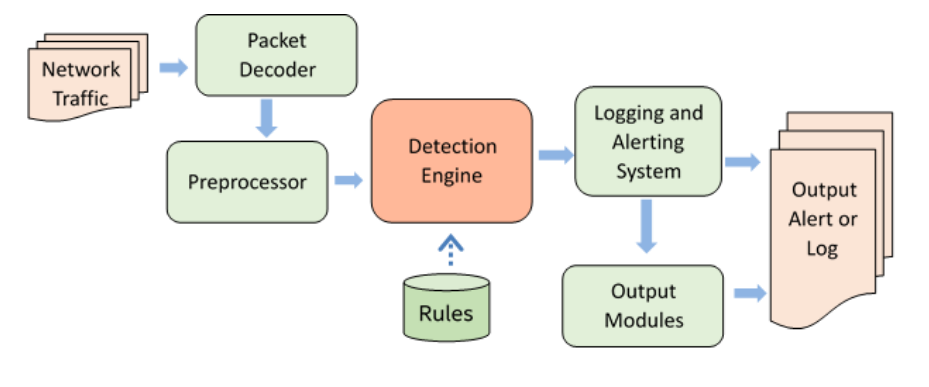
\includegraphics[width=0.7\textwidth]{Figuras/nids-funcionamento.png}


    \end{figure}

\end{frame}


\begin{frame}{NIDS: A Limitação da Criptografia e Modos de Sensor}
    \begin{itemize}
        \item \textbf{A Grande Limitação - Criptografia:}
              \begin{itemize}
                  \item Com o uso crescente de criptografia (ex: TLS/SSL), os NIDS \textbf{perderam o acesso ao conteúdo (payload)} significativo do tráfego.
                  \item Isso \textbf{prejudica (hindering)} sua capacidade de funcionar bem (ex: não podem ver comandos maliciosos dentro de uma sessão HTTPS).
                  \item \textbf{Conclusão:} NIDS são importantes, mas só podem formar \textbf{parte} da solução (Defesa em Profundidade).
              \end{itemize}

        \item \textbf{Tipos de Sensores de Rede (Modos):}

        \item \textbf{1. Sensor Inline }
              \begin{itemize}
                  \item Inserido em um segmento de rede; o tráfego \textbf{deve passar através} do sensor.
                  \item (Pode ser combinado com um firewall ou switch).
                  \item \textbf{Vantagem (IPS):} Permite \textbf{bloquear} um ataque quando detectado (atuando como IDS e \textbf{IPS} - Intrusion Prevention System).
              \end{itemize}

        \item \textbf{2. Sensor Passivo }
              \begin{itemize}
                  \item (Mais comum).
                  \item Monitora uma \textbf{cópia} do tráfego de rede; o tráfego real \textit{não} passa pelo dispositivo.
                  \item \textbf{Vantagem:} Mais eficiente, pois não adiciona um passo de manuseio extra (não contribui para o atraso/delay dos pacotes).
              \end{itemize}
    \end{itemize}
\end{frame}

\begin{frame}{NIDS: Configuração Passiva e Sensores Wireless (WIDS)}
    \begin{itemize}
        \item \textbf{Configuração Típica}
              \begin{itemize}
                  \item O sensor se conecta ao meio (ex: cabo de fibra óptica) através de um \textbf{"tap"} (derivação física).
                  \item O "tap" fornece ao sensor uma \textbf{cópia} de todo o tráfego da rede.
                  \item \textbf{Uso de Placas de Rede:}
                        \begin{itemize}
                            \item \textbf{NIC 1 (Coleta):} Conectada ao "tap". Geralmente \textbf{não possui um endereço IP}. Apenas coleta todo o tráfego (modo promíscuo).
                            \item \textbf{NIC 2 (Gerenciamento):} Conectada à rede \textbf{com um endereço IP}. Permite ao sensor se comunicar com o servidor de gerenciamento NIDS.
                        \end{itemize}
              \end{itemize}

        \item \textbf{Distinção: Sensores Wireless}
              \begin{itemize}
                  \item Pode ser \textit{inline} (incorporado em um Access Point - AP) ou \textit{passivo} (monitorando o tráfego "pelo ar").
                  \item \textbf{Função:} Apenas sensores wireless podem analisar o tráfego de \textbf{protocolo wireless} e detectar ataques específicos (ex: DoS wireless, sequestro de sessão, AP falso).
                  \item \textbf{WIDS (Wireless IDS):} Um NIDS focado exclusivamente em redes sem fio.
              \end{itemize}
    \end{itemize}
\end{frame}

\begin{frame}{Honeypots: Definição e Propósito}
    \begin{itemize}
        \item Honeypots (Potes de Mel) são \textbf{sistemas-isca (decoy systems)}.
        \item São projetados para \textbf{atrair (lure)} um atacante potencial para \textbf{longe} dos sistemas críticos.

        \item \textbf{Três Objetivos Principais:}
              \begin{itemize}
                  \item \textbf{1. Desviar (Divert):} Desviar um atacante de acessar sistemas críticos.
                  \item \textbf{2. Coletar Informações:} Coletar dados sobre a atividade do atacante (técnicas, ferramentas).
                  \item \textbf{3. Ganhar Tempo (Encourage):} Encorajar o atacante a ficar no sistema tempo suficiente para que os administradores possam responder.
              \end{itemize}

        \item \textbf{A Lógica Fundamental:}
              \begin{itemize}
                  \item O honeypot é preenchido com \textbf{informações fabricadas} (que parecem valiosas, mas um usuário legítimo nunca acessaria).
                  \item \textbf{Qualquer acesso} ao honeypot é, por definição, \textbf{suspeito}.
                  \item O sistema é instrumentado com monitores e loggers sensíveis.
                  \item Como o ataque "parece" ser bem-sucedido, os admins podem rastrear o atacante sem expor sistemas produtivos.
              \end{itemize}
    \end{itemize}
\end{frame}

\begin{frame}{Honeypots: Tipos de Interação (Low vs. High)}
    \begin{itemize}
        \item \textbf{Valor do Honeypot:} É um recurso sem valor de produção. Não há razão legítima para interação.
              \begin{itemize}
                  \item Qualquer comunicação \textit{de entrada} (inbound) é (provavelmente) uma sonda, scan ou ataque.
                  \item Se um honeypot inicia comunicação \textit{de saída} (outbound), ele (provavelmente) foi comprometido.
              \end{itemize}

        \item \textbf{Classificação (Nível de Interação):}

        \item \textbf{1. Low Interaction Honeypot (Baixa Interação)}
              \begin{itemize}
                  \item Um pacote de software que \textbf{EMULA} serviços ou sistemas (ex: finge ser um servidor FTP).
                  \item Fornece uma interação inicial realista, mas \textbf{não executa} a versão completa dos serviços.
              \end{itemize}

        \item \textbf{2. High Interaction Honeypot (Alta Interação)}
              \begin{itemize}
                  \item É um \textbf{sistema real}: S.O. completo, serviços e aplicações reais.
                  \item O sistema é instrumentado (monitorado) e colocado onde os atacantes podem acessá-lo.
              \end{itemize}
    \end{itemize}
\end{frame}

\begin{frame}{Trade-offs (High vs. Low) e Honeynets}
    \begin{itemize}
        \item \textbf{High Interaction (Vantagem):}
              \begin{itemize}
                  \item Um alvo \textbf{muito mais realista}.
                  \item Pode "ocupar" (prender) um atacante por um período extenso.
              \end{itemize}

        \item \textbf{High Interaction (Desvantagens / Riscos):}
              \begin{itemize}
                  \item Requer \textbf{significativamente mais recursos} (é um S.O. real).
                  \item \textbf{RISCO:} Se for comprometido, pode ser usado pelo atacante para iniciar ataques contra \textbf{outros sistemas} (na Internet).
                  \item Isso pode resultar em problemas \textbf{legais} ou de \textbf{reputação} indesejados para a organização.
              \end{itemize}

        \item \textbf{Low Interaction (Vantagem):}
              \begin{itemize}
                  \item Suficiente para detectar estágios iniciais do ataque (scan, probe) e alertar (como componente de um IDS distribuído).
              \end{itemize}

        \item \textbf{Honeynet (Rede Honeypot):}
              \begin{itemize}
                  \item Esforços recentes ("The Honeynet Project") focam em construir \textbf{redes inteiras} de honeypots que emulam uma empresa (com tráfego simulado).
              \end{itemize}
    \end{itemize}
\end{frame}

\begin{frame}{Implantação (Deployment) de Honeypots}
    \begin{itemize}
        \item A localização depende dos objetivos (tipo de info a coletar) e do nível de risco tolerado.
    \end{itemize}



    \begin{itemize}
        \item \textbf{1. Externo} (Internet, antes do firewall)
        \item \textbf{2. DMZ} (Rede de Serviços, entre firewalls)
        \item \textbf{3. Interno} (Rede Corporativa, após o firewall)
    \end{itemize}
\end{frame}

\begin{frame}{Implantação: Posição 1 (Externa)}
    \begin{itemize}
        \item \textbf{Localização:} Na Internet, \textbf{antes} do firewall externo.

        \item \textbf{Vantagens:}
              \begin{itemize}
                  \item Útil para rastrear tentativas de conexão a \textbf{IPs não utilizados} (scans).
                  \item \textbf{Não aumenta o risco} para a rede interna (o perigo de um sistema comprometido *atrás* do firewall é evitado).
                  \item \textbf{Reduz "ruído":} Atrai muitos ataques, reduzindo os alertas no firewall e nos sensores IDS internos (facilitando o gerenciamento).
              \end{itemize}

        \item \textbf{Desvantagem:}
              \begin{itemize}
                  \item Pouca ou nenhuma capacidade de capturar \textbf{atacantes internos}.
              \end{itemize}
    \end{itemize}
\end{frame}

\begin{frame}{Implantação: Posição 2 (DMZ)}
    \begin{itemize}
        \item \textbf{Localização:} Na rede de serviços (Web, Mail), ou seja, \textbf{dentro da DMZ} (entre o firewall externo e o interno).

        \item \textbf{Vantagem (Implícita):}
              \begin{itemize}
                  \item Monitora ataques direcionados aos serviços públicos (Web, Mail, DNS).
              \end{itemize}

        \item \textbf{Desvantagens (Trade-off):}
              \begin{itemize}
                  \item \textbf{Risco de Contaminação:} O admin deve garantir que os \textit{outros sistemas} (legítimos) na DMZ estejam seguros contra o honeypot (caso ele seja comprometido).
                  \item \textbf{Conflito com Firewall:} O firewall (externo) tipicamente \textbf{bloqueia} tráfego desnecessário para a DMZ (ex: permite só porta 80, 443).
                  \item \textbf{Dilema:} O admin deve (1) \textbf{abrir o firewall} (aumentando o risco) ou (2) \textbf{limitar a eficácia} do honeypot (que não verá os ataques bloqueados).
              \end{itemize}
    \end{itemize}
\end{frame}

\begin{frame}{Implantação: Posição 3 (Interna) e "Honeyfiles"}
    \begin{itemize}
        \item \textbf{Localização:} Na rede \textbf{totalmente interna}.

        \item \textbf{Vantagens:}
              \begin{itemize}
                  \item Vantagem mais importante: Pode capturar \textbf{ataques internos}.
                  \item Pode detectar um firewall \textbf{mal configurado} (que encaminha tráfego indevido da Internet para a rede interna).
              \end{itemize}

        \item \textbf{Desvantagens (Sérias):}
              \begin{itemize}
                  \item \textbf{Risco Alto:} Se o honeypot for comprometido, ele pode atacar \textbf{outros sistemas internos}.
                  \item (O firewall não bloquearia o tráfego do atacante para o honeypot, pois ele é visto como tráfego "permitido" para o honeypot).
                  \item (Similar à DMZ, o firewall interno precisa de regras de exceção).
              \end{itemize}
              \hrule
        \item \textbf{Tecnologia Relacionada: Honeyfiles}
              \begin{itemize}
                  \item Emulam \textbf{documentos} legítimos (com nomes realistas, ex: "Salarios\_Diretoria.xlsx").
                  \item Atuam como "isca" (bait) para intrusos.
                  \item \textbf{Qualquer acesso} a esses arquivos (que não deveriam ser acessados por usuários legítimos) é considerado \textbf{suspeito}.
              \end{itemize}
    \end{itemize}
\end{frame}



\begin{frame}[fragile]{Regra SNORT}
    \small
    \textbf{Regra Snort:}
    \begin{verbatim}
alert tcp $HOME_NET any -> $EXTERNAL_NET ![7680,1521] 
(msg:"ET P2P BitTorrent peer sync"; 
 flow:established,to_server; 
 content:"|00 00 00 0d 06 00|"; depth:6; 
 threshold: type limit, track by_dst, seconds 300, count 1; 
 reference:url,bitconjurer.org/BitTorrent/protocol.html; 
 classtype:policy-violation; sid:2000334; rev:14; 
 metadata:created_at 2010_07_30, confidence Medium, 
 signature_severity Informational, updated_at 2025_06_30;)
\end{verbatim}
\end{frame}



\begin{frame}{Cabeçalho da Regra}
    \small
    \texttt{alert tcp \$HOME\_NET any -> \$EXTERNAL\_NET ![7680,1521]}

    \begin{itemize}
        \item \textbf{alert}: gera um alerta quando a condição é atendida.
        \item \textbf{tcp}: apenas tráfego TCP.
        \item \textbf{\$HOME\_NET any}: origem na rede interna, qualquer porta.
        \item \textbf{\$EXTERNAL\_NET ![7680,1521]}: destino na rede externa, exceto portas 7680 e 1521.
    \end{itemize}
\end{frame}

\begin{frame}{Opções da Regra (1/2)}
    \small
    \texttt{msg:"ET P2P BitTorrent peer sync"; \\
        flow:established,to\_server; \\
        content:"|00 00 00 0d 06 00|"; depth:6;}

    \begin{itemize}
        \item \textbf{msg:} Mensagem exibida nos logs.
        \item \textbf{flow:established,to\_server:} Só considera conexões TCP já estabelecidas, indo para o servidor.
        \item \textbf{content:} Procura a sequência de bytes \texttt{00 00 00 0d 06 00}.
        \item \textbf{depth:6:} Pesquisa apenas nos primeiros 6 bytes do payload.
    \end{itemize}
\end{frame}

\begin{frame}{Opções da Regra (2/2)}
    \small
    \texttt{threshold: type limit, track by\_dst, seconds 300, count 1; \\
        reference:url,bitconjurer.org/BitTorrent/protocol.html; \\
        classtype:policy-violation; sid:2000334; rev:14;}

    \begin{itemize}
        \item \textbf{threshold:} Evita múltiplos alertas — 1 alerta por destino a cada 300s.
        \item \textbf{reference:} Link para a documentação do protocolo BitTorrent.
        \item \textbf{classtype:} Categoria: violação de política.
        \item \textbf{sid:} Identificador único (2000334).
        \item \textbf{rev:} Revisão nº 14.
    \end{itemize}
\end{frame}